\documentclass[11pt,openright,a4paper]{report}

 %%%%		Importation de tous les packages		%%%%%
\usepackage{tocloft}
\usepackage{graphicx}
\usepackage[utf8]{inputenc}
\usepackage[francais]{babel}
\usepackage{geometry}
\usepackage[T1]{fontenc}
\usepackage{sectsty}
\usepackage{fancyhdr}	% Permet de faire entête et pied de page
\usepackage{tabularx} 	% Pour faire des tableaux
\usepackage{hyperref}	% Pour faire les hyperliens internes
\usepackage{color}
\usepackage[svgnames]{xcolor}
\usepackage{tcolorbox}
\usepackage{tikz}
\usepackage{ifmtarg}
\usepackage{listings}
\usepackage{textcomp}
\usepackage{boxedminipage}
\usepackage[framemethod=default]{mdframed}
\usepackage[
		%shortlop,
		under,
		side,
		%top,
		center,
		bottom,
	]{photo}
\usepackage{indentfirst}
\selectlanguage{francais}
%%%%%%%%%%%%%%%%%%%%%%%%%%%%%%%%%%%%%%%%%%%%%%%%%%%%%%


 %%%%	Gestion de la dimension du document		%%%%%
	\oddsidemargin 0.8cm
	\evensidemargin -0.2cm
	\textwidth 16cm
	\textheight 23cm
	\topmargin -0.5cm
%%%%%%%%%%%%%%%%%%%%%%%%%%%%%%%%%%%%%%%%%%%%%%%%%%%%%%


 %%%%	Préparation des nouvelles commandes		%%%%%
\renewcommand{\familydefault}{\sfdefault}

% Couleur et définition du thème chapter
\definecolor{monbleu}{HTML}{4E83A2}
\newcommand{\mychapter}[1]{\textcolor{monbleu}{\chapter{#1}}}

% Couleur et définition du thème section
\definecolor{monvert}{HTML}{0BA486}
\newcommand{\mysection}[1]{\textcolor{monvert}{\section{#1}}}

% Couleur et définition du thème subsection
\definecolor{monorange}{HTML}{E95D0F}
\newcommand{\mysubsection}[1]{\textcolor{monorange}{\subsection{#1}}}
%%%%%%%%%%%%%%%%%%%%%%%%%%%%%%%%%%%%%%%%%%%%%%%%%%%%%%%
			
			
			
%%%%		Pour mettre du code dans des boites		 %%%%%
\makeatletter				
	\newcommand{\mybox}[1]{%
  		\setbox0=\hbox{#1}%
  		\setlength{\@tempdima}{\dimexpr\wd0+13pt}%
  		\begin{tcolorbox}[	colframe=black!40,
  							boxrule=0.5pt,
  							arc=4pt,
      						left=6pt,
      						right=6pt,
      						top=6pt,
      						bottom=6pt,
      						boxsep=0pt,
      						width=16cm
      					]
    			#1
  		\end{tcolorbox}
}
\makeatother
%%%%%%%%%%%%%%%%%%%%%%%%%%%%%%%%%%%%%%%%%%%%%%%%%%%%%%%



%%%%		Pour coloriser les codes PHP ou autres		 %%%%%
\lstset{language=PHP,
    		basicstyle=\ttfamily\small,
    		breaklines=false,
    		prebreak=\raisebox{0ex}[0ex][0ex]{\ensuremath{\hookleftarrow}},
    		frame=lines,
    		showtabs=false,
    		showspaces=false,
    		showstringspaces=false,
    		keywordstyle=\color{red}\bfseries,
    		stringstyle=\color{green!50!black},
    		commentstyle=\color{gray}\itshape,
    		numbers=left,
    		captionpos=t,
    		escapeinside={\%*}{*)}
		}
%%%%%%%%%%%%%%%%%%%%%%%%%%%%%%%%%%%%%%%%%%%%%%%%%%%%%%%%%%%



%%%%%%%%		 	table of contents config			%%%%%%%%

\tocloftpagestyle{empty}
\setcounter{tocdepth}{1}
%%%%%%%%%%%%%%%%%%%%%%%%%%%%%%%%%%%%%%%%%%%%%%%%%%%%%%%%%



%%%%%%%%		 	Définition des entêtes et pieds de page			%%%%%%%%
\pagestyle{fancy}
	\lhead[\fancyplain{}{\raggedright\slshape\leftmark}]{}
	\chead{}
	\rhead[]{\fancyplain{}{\raggedleft\slshape\rightmark}}
	\fancyfoot[L]{Freddy Dubois}
	\rfoot[Licence Professionnelle - IUT Orléans]{Licence Professionnelle - IUT Orléans}
\fancypagestyle{plain} %Pour avoir le pied de page sur les première pages des chapitres
%%%%%%%%%%%%%%%%%%%%%%%%%%%%%%%%%%%%%%%%%%%%%%%%%%%%%%%%%%%%%%%%%%%%%%%%%

\begin{document}

%%%%%%%%%%		Page de garde		%%%%%%%%%%
	\begin{titlepage}
		\begin{Large}
		\baselineskip=7mm
		\noindent
			
\includegraphics[height=2cm]{../images/logo.png}
			\hfill
			
\includegraphics[height=2cm]{../images/logo_IUT}
			\vskip 30mm
			\begin{center}
				\rule{\textwidth}{0.5 mm}\\
				{\huge\sffamily\bfseries\baselineskip=1cm
					Sujet
				\par}
				\rule{\textwidth}{0.5 mm}\\
				{\Large\sffamily\bfseries 
					Rapport de stage/TER/...
				}
					\vskip 20mm
				Freddy DUBOIS
					\vskip 5mm
				17 février au 13 juin 2014
					\vskip 5mm
				Année universitaire 2013 - 2014
					\vfill
					\vskip 45mm
				\begin{tabular}{l l p{4cm} l l}
					 Tuteur : Olivier ZOÏS		&	&	&	Tuteur : Enseignant	
				\end{tabular}
			\end{center}
		\end{Large}
	\end{titlepage}

%%%%%%%%%%%%%%%%%%%%%%%%%%%%%%%%%%%%%%%%%%%%%%%


%%%%%%%%%%%		Contenu du mémoire	%%%%%%%%%%
\cleardoublepage
\section*{Remerciements}
\noindent
\phantomsection
\addcontentsline{toc}{section}{Remerciements}


Je tiens à remercier toute l'équipe informatique ainsi que M.Olivier ZOÏS mon maître de stage, directeur informatique 
au sein d'\interlog  pour m’avoir accepté en stage et de m’avoir
offert la possibilité d’une expérience professionnelle.\\


Je tiens également à remercier mon tuteur de stage et toute l’équipe enseignante qui
m’ont tous permis d’obtenir les connaissances nécessaires pour intégrer le milieu
professionnel.\\


Enfin, je remercie ma femme qui m’a soutenu tout au long de cette année universitaire
mais également dans mon projet de reconversion professionnelle.

\newpage



 % Mettre ici les remerciements

\tableofcontents			% Table des matières

\addcontentsline{toc}{chapter}{Table des mati\`eres}
\mychapter{Introduction}


Etudiant en Licence Professionnelle Réseaux Télécoms option Web et Mobile, 
j’ai réalisé un stage de seize semaines au sein d'Interlog Services à Orléans du 15 février au 7 juin 2014.\\

Durant mon stage, j’ai eu pour mission de développer des améliorations d'applications existantes
dans l'entreprise.\\


Dans un premier temps, je présenterai l’établissement qui m’a accueilli. L’exposition
des sujets de mon stage se fera dans un second temps, qui sera suivi par la présentation de
l’environnement de travail dans lequel les applications ont été développées. Une quatrième
partie sera consacrée au travail réalisé. Le bilan du stage conclura ce rapport.




\mychapter{Présentation}

%\begin{figure}[!h] % option !h pour dire que l'image sera à cet endroit
%	\centering
%	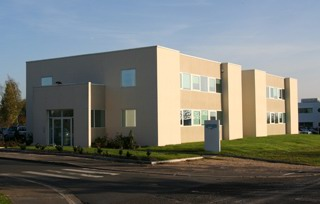
\includegraphics[scale=0.5]{../images/siege_interlog.jpg}
%	\caption{Siège social, Interlog Services à Orléans}
%	\label{Siege interlog}
%\end{figure}

\mysection{Interlog Services}

\begin{photo}[!h]
	\centering
	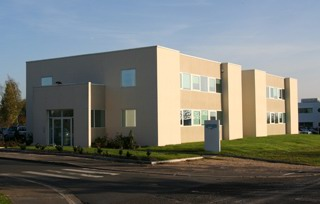
\includegraphics[scale=0.5]{../images/siege_interlog.jpg}
	\caption{Siège social, Interlog Services à Orléans}
\end{photo}

\mysubsection{Présentation de l'entreprise}
\textit{Interlog Service}, anciennement \textit{ipseurope}, a été créé en 1999. Il s'agit de la première société à proposer sur le continent européen des audits de factures de transport.\\

La société intervient au coeur de la \og Supply-Chain\fg \footnote{chaîne logistique}  et propose des prestations permettant des gains non négligeables. Les clients viennent de tous les secteurs d'activités (luxe, agroalimentaire, automobile \ldots).

\mysubsection{La direction}
L'équipe de direction est composée :
\begin{itemize}
\item d'un président,
\item d'une directrice générale et d'un directeur général,
\item d'un directeur commercial,
\item d'un directeur des opérations logistiques,
\item d'un directeur informatique.
\end{itemize}

\mysubsection{Le secteur informatique}
Le secteur informatique est dirigé par le directeur informatique, Monsieur Zoïs. L'équipe de développeurs informatiques est composée de six personnes dont le chef de projets et  cinq développeurs.\\

Le but principal de cette équipe est de développer des applications, elle  met également à jour celles  existant déjà, et règle d'éventuels bugs informatiques. Elle peut aussi, en fonction de la demande du client,  développer de nouvelles fonctionnalités nécessaires à ce dernier.


\mysection{Soutenance}

\mysubsection{Support}

La présentation doit être réalisée en utilisant Beamer.
Il faut compter environ une page de présentation par minute, soit environ 30 pages pour 30 minutes de présentation.
Chaque page doit contenir 

\mysubsection{Oral}

Etapes à suivre :
\begin{enumerate}
\item se présenter
\item sujet, contexte du stage
\item plan de la présentation
\item intro
\item ...
\item conclusion
\end{enumerate}

Recommendations :
\begin{itemize}
\item répéter plusieurs fois en situation
\item regarder l'auditoire
\item bien se placer par rapport à l'auditoire, à l'écran et à l'ordinateur pour éviter de se trouver dos à l'auditoire ou de se déplacer pour cliquer sur le clavier
\item ne pas avoir de papier entre les mains
\item éviter le langage familier
\item ne pas lire la présentation
\end{itemize}


%
\mychapter{Projet}


\mysection{Organisation du projet}
hgdghf


\mysection{Archivage du projet}


%\mychapter{Codage}


\mysection{Rêgles de codage}


\mysubsection{Identifiers}

Noms des classes : 

Noms des fonctions :

Noms des variables :




\mysection{Documentation du code}

doxygen
JE vlshdf;sbvkwuvlsdnfs
cglbilibldkbndfb
dhfhdfj
g,nghjfg
hjfghjk
hjkgh
jh
gkl
ghjkl
jklhjklmhjk:
gs<dv
wfb
bd
bd

\mybox{
%\begin{boxedminipage}[poslb]{15.5cm}
\lstinputlisting[caption={Un hello world},
  				label=hello,
  				tabsize=2,
  				%backgroundcolor=yellow,
  				language=PHP]{../tex/4-code/hello.php}
%\end{boxedminipage}
}
comme le montre \ref{hello}
%\begin{lstlisting}[language=PHP]
%\lstinputlisting{hello.php}
%\end{lstlisting}



doxygen
JE vlshdf;sbvkwuvlsdnfs
cglbilibldkbndfb
dhfhdfj
g,nghjfg
hjfghjk
hjkgh
jh
gkl
ghjkl
jklhjklmhjk:
gs<dv
wfb
bd
bd
doxygen
JE vlshdf;sbvkwuvlsdnfs
cglbilibldkbndfb
dhfhdfj
g,nghjfg
hjfghjk
hjkgh
jh
gkl
ghjkl
jklhjklmhjk:
gs<dv
wfb
bd
bd
doxygen
JE vlshdf;sbvkwuvlsdnfs
cglbilibldkbndfb
dhfhdfj
g,nghjfg
hjfghjk
hjkgh
jh
gkl
ghjkl
jklhjklmhjk:
gs<dv
wfb
bd
bd
doxygen
JE vlshdf;sbvkwuvlsdnfs
cglbilibldkbndfb
dhfhdfj
g,nghjfg
hjfghjk
hjkgh
jh
gkl
ghjkl
jklhjklmhjk:
gs<dv
wfb
bd
bd
doxygen
JE vlshdf;sbvkwuvlsdnfs
cglbilibldkbndfb
dhfhdfj
g,nghjfg
hjfghjk
hjkgh
jh
gkl
ghjkl
jklhjklmhjk:
gs<dv
wfb
bd
bd
doxygen
JE vlshdf;sbvkwuvlsdnfs
cglbilibldkbndfb
dhfhdfj
g,nghjfg
hjfghjk
hjkgh
jh
gkl
ghjkl
jklhjklmhjk:
gs<dv
wfb
bd
bd
doxygen
JE vlshdf;sbvkwuvlsdnfs
cglbilibldkbndfb
dhfhdfj
g,nghjfg
hjfghjk
hjkgh
jh
gkl
ghjkl
jklhjklmhjk:
gs<dv
wfb
bd
bd
doxygen
JE vlshdf;sbvkwuvlsdnfs
cglbilibldkbndfb
dhfhdfj
g,nghjfg
hjfghjk
hjkgh
jh
gkl
ghjkl
jklhjklmhjk:
gs<dv
wfb
bd
bd
doxygen
JE vlshdf;sbvkwuvlsdnfs
cglbilibldkbndfb
dhfhdfj
g,nghjfg
hjfghjk
hjkgh
jh
gkl
ghjkl
jklhjklmhjk:
gs<dv
wfb
bd
bd
doxygen
JE vlshdf;sbvkwuvlsdnfs
cglbilibldkbndfb
dhfhdfj
g,nghjfg
hjfghjk
hjkgh
jh
gkl
ghjkl
jklhjklmhjk:
gs<dv
wfb
bd
bd
doxygen
JE vlshdf;sbvkwuvlsdnfs
cglbilibldkbndfb
dhfhdfj
g,nghjfg
hjfghjk
hjkgh
jh
gkl
ghjkl
jklhjklmhjk:
gs<dv
wfb
bd
bddoxygen
JE vlshdf;sbvkwuvlsdnfs
cglbilibldkbndfb
dhfhdfj
g,nghjfg
hjfghjk
hjkgh
jh
gkl
ghjkl
jklhjklmhjk:
gs<dv
wfb
bd
bddoxygen
JE vlshdf;sbvkwuvlsdnfs
cglbilibldkbndfb
dhfhdfj
g,nghjfg
hjfghjk
hjkgh
jh
gkl
ghjkl
jklhjklmhjk:
gs<dv
wfb
bd
bddoxygen
JE vlshdf;sbvkwuvlsdnfs
cglbilibldkbndfb
dhfhdfj
g,nghjfg
hjfghjk
hjkgh
jh
gkl
ghjkl
jklhjklmhjk:
gs<dv
wfb
bd
bddoxygen
JE vlshdf;sbvkwuvlsdnfs
cglbilibldkbndfb
dhfhdfj
g,nghjfg
hjfghjk
hjkgh
jh
gkl
ghjkl
jklhjklmhjk:
gs<dv
wfb
bd
bddoxygen
JE vlshdf;sbvkwuvlsdnfs
cglbilibldkbndfb
dhfhdfj
g,nghjfg
hjfghjk
hjkgh
jh
gkl
ghjkl
jklhjklmhjk:
gs<dv
wfb
bd
bddoxygen
JE vlshdf;sbvkwuvlsdnfs
cglbilibldkbndfb
dhfhdfj
g,nghjfg
hjfghjk
hjkgh
jh
gkl
ghjkl
jklhjklmhjk:
gs<dv
wfb
bd
bddoxygen
JE vlshdf;sbvkwuvlsdnfs
cglbilibldkbndfb
dhfhdfj
g,nghjfg
hjfghjk
hjkgh
jh
gkl
ghjkl
jklhjklmhjk:
gs<dv
wfb
bd
bddoxygen
JE vlshdf;sbvkwuvlsdnfs
cglbilibldkbndfb
dhfhdfj
g,nghjfg
hjfghjk
hjkgh
jh
gkl
ghjkl
jklhjklmhjk:
gs<dv
wfb
bd
bddoxygen
JE vlshdf;sbvkwuvlsdnfs
cglbilibldkbndfb
dhfhdfj
g,nghjfg
hjfghjk
hjkgh
jh
gkl
ghjkl
jklhjklmhjk:
gs<dv
wfb
bd
bddoxygen
JE vlshdf;sbvkwuvlsdnfs
cglbilibldkbndfb
dhfhdfj
g,nghjfg
hjfghjk
hjkgh
jh
gkl
ghjkl
jklhjklmhjk:
gs<dv
wfb
bd
bddoxygen
JE vlshdf;sbvkwuvlsdnfs
cglbilibldkbndfb
dhfhdfj
g,nghjfg
hjfghjk
hjkgh
jh
gkl
ghjkl
jklhjklmhjk:
gs<dv
wfb
bd
bddoxygen
JE vlshdf;sbvkwuvlsdnfs
cglbilibldkbndfb
dhfhdfj
g,nghjfg
hjfghjk
hjkgh
jh
gkl
ghjkl
jklhjklmhjk:
gs<dv
wfb
bd
bddoxygen
JE vlshdf;sbvkwuvlsdnfs
cglbilibldkbndfb
dhfhdfj
g,nghjfg
hjfghjk
hjkgh
jh
gkl
ghjkl
jklhjklmhjk:
gs<dv
wfb
bd
bddoxygen
JE vlshdf;sbvkwuvlsdnfs
cglbilibldkbndfb
dhfhdfj
g,nghjfg
hjfghjk
hjkgh
jh
gkl
ghjkl
jklhjklmhjk:
gs<dv
wfb
bd
bddoxygen
JE vlshdf;sbvkwuvlsdnfs
cglbilibldkbndfb
dhfhdfj
g,nghjfg
hjfghjk
hjkgh
jh
gkl
ghjkl
jklhjklmhjk:
gs<dv
wfb
bd
bddoxygen
JE vlshdf;sbvkwuvlsdnfs
cglbilibldkbndfb
dhfhdfj
g,nghjfg
hjfghjk
hjkgh
jh
gkl
ghjkl
jklhjklmhjk:
gs<dv
wfb
bd
bddoxygen
JE vlshdf;sbvkwuvlsdnfs
cglbilibldkbndfb
dhfhdfj
g,nghjfg
hjfghjk
hjkgh
jh
gkl
ghjkl
jklhjklmhjk:
gs<dv
wfb
bd
bddoxygen
JE vlshdf;sbvkwuvlsdnfs
cglbilibldkbndfb
dhfhdfj
g,nghjfg
hjfghjk
hjkgh
jh
gkl
ghjkl
jklhjklmhjk:
gs<dv
wfb
bd
bddoxygen
JE vlshdf;sbvkwuvlsdnfs
cglbilibldkbndfb
dhfhdfj
g,nghjfg
hjfghjk
hjkgh
jh
gkl
ghjkl
jklhjklmhjk:
gs<dv
wfb
bd
bddoxygen
JE vlshdf;sbvkwuvlsdnfs
cglbilibldkbndfb
dhfhdfj
g,nghjfg
hjfghjk
hjkgh
jh
gkl
ghjkl
jklhjklmhjk:
gs<dv
wfb
bd
bddoxygen
JE vlshdf;sbvkwuvlsdnfs
cglbilibldkbndfb
dhfhdfj
g,nghjfg
hjfghjk
hjkgh
jh
gkl
ghjkl
jklhjklmhjk:
gs<dv
wfb
bd
bddoxygen
JE vlshdf;sbvkwuvlsdnfs
cglbilibldkbndfb
dhfhdfj
g,nghjfg
hjfghjk
hjkgh
jh
gkl
ghjkl
jklhjklmhjk:
gs<dv
wfb
bd
bddoxygen
JE vlshdf;sbvkwuvlsdnfs
cglbilibldkbndfb
dhfhdfj
g,nghjfg
hjfghjk
hjkgh
jh
gkl
ghjkl
jklhjklmhjk:
gs<dv
wfb
bd
bddoxygen
JE vlshdf;sbvkwuvlsdnfs
cglbilibldkbndfb
dhfhdfj
g,nghjfg
hjfghjk
hjkgh
jh
gkl
ghjkl
jklhjklmhjk:
gs<dv
wfb
bd
bddoxygen
JE vlshdf;sbvkwuvlsdnfs
cglbilibldkbndfb
dhfhdfj
g,nghjfg
hjfghjk
hjkgh
jh
gkl
ghjkl
jklhjklmhjk:
gs<dv
wfb
bd
bddoxygen
JE vlshdf;sbvkwuvlsdnfs
cglbilibldkbndfb
dhfhdfj
g,nghjfg
hjfghjk
hjkgh
jh
gkl
ghjkl
jklhjklmhjk:
gs<dv
wfb
bd
bddoxygen
JE vlshdf;sbvkwuvlsdnfs
cglbilibldkbndfb
dhfhdfj
g,nghjfg
hjfghjk
hjkgh
jh
gkl
ghjkl
jklhjklmhjk:
gs<dv
wfb
bd
bddoxygen
JE vlshdf;sbvkwuvlsdnfs
cglbilibldkbndfb
dhfhdfj
g,nghjfg
hjfghjk
hjkgh
jh
gkl
ghjkl
jklhjklmhjk:
gs<dv
wfb
bd
bddoxygen
JE vlshdf;sbvkwuvlsdnfs
cglbilibldkbndfb
dhfhdfj
g,nghjfg
hjfghjk
hjkgh
jh
gkl
ghjkl
jklhjklmhjk:
gs<dv
wfb
bd
bddoxygen
JE vlshdf;sbvkwuvlsdnfs
cglbilibldkbndfb
dhfhdfj
g,nghjfg
hjfghjk
hjkgh
jh
gkl
ghjkl
jklhjklmhjk:
gs<dv
wfb
bd
bddoxygen
JE vlshdf;sbvkwuvlsdnfs
cglbilibldkbndfb
dhfhdfj
g,nghjfg
hjfghjk
hjkgh
jh
gkl
ghjkl
jklhjklmhjk:
gs<dv
wfb
bd
bddoxygen
JE vlshdf;sbvkwuvlsdnfs
cglbilibldkbndfb
dhfhdfj
g,nghjfg
hjfghjk
hjkgh
jh
gkl
ghjkl
jklhjklmhjk:
gs<dv
wfb
bd
bddoxygen
JE vlshdf;sbvkwuvlsdnfs
cglbilibldkbndfb
dhfhdfj
g,nghjfg
hjfghjk
hjkgh
jh
gkl
ghjkl
jklhjklmhjk:
gs<dv
wfb
bd
bddoxygen
JE vlshdf;sbvkwuvlsdnfs
cglbilibldkbndfb
dhfhdfj
g,nghjfg
hjfghjk
hjkgh
jh
gkl
ghjkl
jklhjklmhjk:
gs<dv
wfb
bd
bddoxygen
JE vlshdf;sbvkwuvlsdnfs
cglbilibldkbndfb
dhfhdfj
g,nghjfg
hjfghjk
hjkgh
jh
gkl
ghjkl
jklhjklmhjk:
gs<dv
wfb
bd
bddoxygen
JE vlshdf;sbvkwuvlsdnfs
cglbilibldkbndfb
dhfhdfj
g,nghjfg
hjfghjk
hjkgh
jh
gkl
ghjkl
jklhjklmhjk:
gs<dv
wfb
bd
bddoxygen
JE vlshdf;sbvkwuvlsdnfs
cglbilibldkbndfb
dhfhdfj
g,nghjfg
hjfghjk
hjkgh
jh
gkl
ghjkl
jklhjklmhjk:
gs<dv
wfb
bd
bddoxygen
JE vlshdf;sbvkwuvlsdnfs
cglbilibldkbndfb
dhfhdfj
g,nghjfg
hjfghjk
hjkgh
jh
gkl
ghjkl
jklhjklmhjk:
gs<dv
wfb
bd
bddoxygen
JE vlshdf;sbvkwuvlsdnfs
cglbilibldkbndfb
dhfhdfj
g,nghjfg
hjfghjk
hjkgh
jh
gkl
ghjkl
jklhjklmhjk:
gs<dv
wfb
bd
bddoxygen
JE vlshdf;sbvkwuvlsdnfs
cglbilibldkbndfb
dhfhdfj
g,nghjfg
hjfghjk
hjkgh
jh
gkl
ghjkl
jklhjklmhjk:
gs<dv
wfb
bd
bddoxygen
JE vlshdf;sbvkwuvlsdnfs
cglbilibldkbndfb
dhfhdfj
g,nghjfg
hjfghjk
hjkgh
jh
gkl
ghjkl
jklhjklmhjk:
gs<dv
wfb
bd
bddoxygen
JE vlshdf;sbvkwuvlsdnfs
cglbilibldkbndfb
dhfhdfj
g,nghjfg
hjfghjk
hjkgh
jh
gkl
ghjkl
jklhjklmhjk:
gs<dv
wfb
bd
bddoxygen
JE vlshdf;sbvkwuvlsdnfs
cglbilibldkbndfb
dhfhdfj
g,nghjfg
hjfghjk
hjkgh
jh
gkl
ghjkl
jklhjklmhjk:
gs<dv
wfb
bd
bddoxygen
JE vlshdf;sbvkwuvlsdnfs
cglbilibldkbndfb
dhfhdfj
g,nghjfg
hjfghjk
hjkgh
jh
gkl
ghjkl
jklhjklmhjk:
gs<dv
wfb
bd
bddoxygen
JE vlshdf;sbvkwuvlsdnfs
cglbilibldkbndfb
dhfhdfj
g,nghjfg
hjfghjk
hjkgh
jh
gkl
ghjkl
jklhjklmhjk:
gs<dv
wfb
bd
bddoxygen
JE vlshdf;sbvkwuvlsdnfs
cglbilibldkbndfb
dhfhdfj
g,nghjfg
hjfghjk
hjkgh
jh
gkl
ghjkl
jklhjklmhjk:
gs<dv
wfb
bd
bddoxygen
JE vlshdf;sbvkwuvlsdnfs
cglbilibldkbndfb
dhfhdfj
g,nghjfg
hjfghjk
hjkgh
jh
gkl
ghjkl
jklhjklmhjk:
gs<dv
wfb
bd
bddoxygen
JE vlshdf;sbvkwuvlsdnfs
cglbilibldkbndfb
dhfhdfj
g,nghjfg
hjfghjk
hjkgh
jh
gkl
ghjkl
jklhjklmhjk:
gs<dv
wfb
bd
bddoxygen
JE vlshdf;sbvkwuvlsdnfs
cglbilibldkbndfb
dhfhdfj
g,nghjfg
hjfghjk
hjkgh
jh
gkl
ghjkl
jklhjklmhjk:
gs<dv
wfb
bd
bddoxygen
JE vlshdf;sbvkwuvlsdnfs
cglbilibldkbndfb
dhfhdfj
g,nghjfg
hjfghjk
hjkgh
jh
gkl
ghjkl
jklhjklmhjk:
gs<dv
wfb
bd
bddoxygen
JE vlshdf;sbvkwuvlsdnfs
cglbilibldkbndfb
dhfhdfj
g,nghjfg
hjfghjk
hjkgh
jh
gkl
ghjkl
jklhjklmhjk:
gs<dv
wfb
bd
bddoxygen
JE vlshdf;sbvkwuvlsdnfs
cglbilibldkbndfb
dhfhdfj
g,nghjfg
hjfghjk
hjkgh
jh
gkl
ghjkl
jklhjklmhjk:
gs<dv
wfb
bd
bddoxygen
JE vlshdf;sbvkwuvlsdnfs
cglbilibldkbndfb
dhfhdfj
g,nghjfg
hjfghjk
hjkgh
jh
gkl
ghjkl
jklhjklmhjk:
gs<dv
wfb
bd
bddoxygen
JE vlshdf;sbvkwuvlsdnfs
cglbilibldkbndfb
dhfhdfj
g,nghjfg
hjfghjk
hjkgh
jh
gkl
ghjkl
jklhjklmhjk:
gs<dv
wfb
bd
bddoxygen
JE vlshdf;sbvkwuvlsdnfs
cglbilibldkbndfb
dhfhdfj
g,nghjfg
hjfghjk
hjkgh
jh
gkl
ghjkl
jklhjklmhjk:
gs<dv
wfb
bd
bddoxygen
JE vlshdf;sbvkwuvlsdnfs
cglbilibldkbndfb
dhfhdfj
g,nghjfg
hjfghjk
hjkgh
jh
gkl
ghjkl
jklhjklmhjk:
gs<dv
wfb
bd
bddoxygen
JE vlshdf;sbvkwuvlsdnfs
cglbilibldkbndfb
dhfhdfj
g,nghjfg
hjfghjk
hjkgh
jh
gkl
ghjkl
jklhjklmhjk:
gs<dv
wfb
bd
bddoxygen
JE vlshdf;sbvkwuvlsdnfs
cglbilibldkbndfb
dhfhdfj
g,nghjfg
hjfghjk
hjkgh
jh
gkl
ghjkl
jklhjklmhjk:
gs<dv
wfb
bd
bddoxygen
JE vlshdf;sbvkwuvlsdnfs
cglbilibldkbndfb
dhfhdfj
g,nghjfg
hjfghjk
hjkgh
jh
gkl
ghjkl
jklhjklmhjk:
gs<dv
wfb
bd
bddoxygen
JE vlshdf;sbvkwuvlsdnfs
cglbilibldkbndfb
dhfhdfj
g,nghjfg
hjfghjk
hjkgh
jh
gkl
ghjkl
jklhjklmhjk:
gs<dv
wfb
bd
bddoxygen
JE vlshdf;sbvkwuvlsdnfs
cglbilibldkbndfb
dhfhdfj
g,nghjfg
hjfghjk
hjkgh
jh
gkl
ghjkl
jklhjklmhjk:
gs<dv
wfb
bd
bddoxygen
JE vlshdf;sbvkwuvlsdnfs
cglbilibldkbndfb
dhfhdfj
g,nghjfg
hjfghjk
hjkgh
jh
gkl
ghjkl
jklhjklmhjk:
gs<dv
wfb
bd
bddoxygen
JE vlshdf;sbvkwuvlsdnfs
cglbilibldkbndfb
dhfhdfj
g,nghjfg
hjfghjk
hjkgh
jh
gkl
ghjkl
jklhjklmhjk:
gs<dv
wfb
bd
bddoxygen
JE vlshdf;sbvkwuvlsdnfs
cglbilibldkbndfb
dhfhdfj
g,nghjfg
hjfghjk
hjkgh
jh
gkl
ghjkl
jklhjklmhjk:
gs<dv
wfb
bd
bddoxygen
JE vlshdf;sbvkwuvlsdnfs
cglbilibldkbndfb
dhfhdfj
g,nghjfg
hjfghjk
hjkgh
jh
gkl
ghjkl
jklhjklmhjk:
gs<dv
wfb
bd
bddoxygen
JE vlshdf;sbvkwuvlsdnfs
cglbilibldkbndfb
dhfhdfj
g,nghjfg
hjfghjk
hjkgh
jh
gkl
ghjkl
jklhjklmhjk:
gs<dv
wfb
bd
bddoxygen
JE vlshdf;sbvkwuvlsdnfs
cglbilibldkbndfb
dhfhdfj
g,nghjfg
hjfghjk
hjkgh
jh
gkl
ghjkl
jklhjklmhjk:
gs<dv
wfb
bd
bddoxygen
JE vlshdf;sbvkwuvlsdnfs
cglbilibldkbndfb
dhfhdfj
g,nghjfg
hjfghjk
hjkgh
jh
gkl
ghjkl
jklhjklmhjk:
gs<dv
wfb
bd
bddoxygen
JE vlshdf;sbvkwuvlsdnfs
cglbilibldkbndfb
dhfhdfj
g,nghjfg
hjfghjk
hjkgh
jh
gkl
ghjkl
jklhjklmhjk:
gs<dv
wfb
bd
bddoxygen
JE vlshdf;sbvkwuvlsdnfs
cglbilibldkbndfb
dhfhdfj
g,nghjfg
hjfghjk
hjkgh
jh
gkl
ghjkl
jklhjklmhjk:
gs<dv
wfb
bd
bddoxygen
JE vlshdf;sbvkwuvlsdnfs
cglbilibldkbndfb
dhfhdfj
g,nghjfg
hjfghjk
hjkgh
jh
gkl
ghjkl
jklhjklmhjk:
gs<dv
wfb
bd
bddoxygen
JE vlshdf;sbvkwuvlsdnfs
cglbilibldkbndfb
dhfhdfj
g,nghjfg
hjfghjk
hjkgh
jh
gkl
ghjkl
jklhjklmhjk:
gs<dv
wfb
bd
bddoxygen
JE vlshdf;sbvkwuvlsdnfs
cglbilibldkbndfb
dhfhdfj
g,nghjfg
hjfghjk
hjkgh
jh
gkl
ghjkl
jklhjklmhjk:
gs<dv
wfb
bd
bddoxygen
JE vlshdf;sbvkwuvlsdnfs
cglbilibldkbndfb
dhfhdfj
g,nghjfg
hjfghjk
hjkgh
jh
gkl
ghjkl
jklhjklmhjk:
gs<dv
wfb
bd
bddoxygen
JE vlshdf;sbvkwuvlsdnfs
cglbilibldkbndfb
dhfhdfj
g,nghjfg
hjfghjk
hjkgh
jh
gkl
ghjkl
jklhjklmhjk:
gs<dv
wfb
bd
bddoxygen
JE vlshdf;sbvkwuvlsdnfs
cglbilibldkbndfb
dhfhdfj
g,nghjfg
hjfghjk
hjkgh
jh
gkl
ghjkl
jklhjklmhjk:
gs<dv
wfb
bd
bddoxygen
JE vlshdf;sbvkwuvlsdnfs
cglbilibldkbndfb
dhfhdfj
g,nghjfg
hjfghjk
hjkgh
jh
gkl
ghjkl
jklhjklmhjk:
gs<dv
wfb
bd
bddoxygen
JE vlshdf;sbvkwuvlsdnfs
cglbilibldkbndfb
dhfhdfj
g,nghjfg
hjfghjk
hjkgh
jh
gkl
ghjkl
jklhjklmhjk:
gs<dv
wfb
bd
bddoxygen
JE vlshdf;sbvkwuvlsdnfs
cglbilibldkbndfb
dhfhdfj
g,nghjfg
hjfghjk
hjkgh
jh
gkl
ghjkl
jklhjklmhjk:
gs<dv
wfb
bd
bddoxygen
JE vlshdf;sbvkwuvlsdnfs
cglbilibldkbndfb
dhfhdfj
g,nghjfg
hjfghjk
hjkgh
jh
gkl
ghjkl
jklhjklmhjk:
gs<dv
wfb
bd
bddoxygen
JE vlshdf;sbvkwuvlsdnfs
cglbilibldkbndfb
dhfhdfj
g,nghjfg
hjfghjk
hjkgh
jh
gkl
ghjkl
jklhjklmhjk:
gs<dv
wfb
bd
bddoxygen
JE vlshdf;sbvkwuvlsdnfs
cglbilibldkbndfb
dhfhdfj
g,nghjfg
hjfghjk
hjkgh
jh
gkl
ghjkl
jklhjklmhjk:
gs<dv
wfb
bd
bddoxygen
JE vlshdf;sbvkwuvlsdnfs
cglbilibldkbndfb
dhfhdfj
g,nghjfg
hjfghjk
hjkgh
jh
gkl
ghjkl
jklhjklmhjk:
gs<dv
wfb
bd
bddoxygen
JE vlshdf;sbvkwuvlsdnfs
cglbilibldkbndfb
dhfhdfj
g,nghjfg
hjfghjk
hjkgh
jh
gkl
ghjkl
jklhjklmhjk:
gs<dv
wfb
bd
bddoxygen
JE vlshdf;sbvkwuvlsdnfs
cglbilibldkbndfb
dhfhdfj
g,nghjfg
hjfghjk
hjkgh
jh
gkl
ghjkl
jklhjklmhjk:
gs<dv
wfb
bd
bddoxygen
JE vlshdf;sbvkwuvlsdnfs
cglbilibldkbndfb
dhfhdfj
g,nghjfg
hjfghjk
hjkgh
jh
gkl
ghjkl
jklhjklmhjk:
gs<dv
wfb
bd
bddoxygen
JE vlshdf;sbvkwuvlsdnfs
cglbilibldkbndfb
dhfhdfj
g,nghjfg
hjfghjk
hjkgh
jh
gkl
ghjkl
jklhjklmhjk:
gs<dv
wfb
bd
bddoxygen
JE vlshdf;sbvkwuvlsdnfs
cglbilibldkbndfb
dhfhdfj
g,nghjfg
hjfghjk
hjkgh
jh
gkl
ghjkl
jklhjklmhjk:
gs<dv
wfb
bd
bddoxygen
JE vlshdf;sbvkwuvlsdnfs
cglbilibldkbndfb
dhfhdfj
g,nghjfg
hjfghjk
hjkgh
jh
gkl
ghjkl
jklhjklmhjk:
gs<dv
wfb
bd
bddoxygen
JE vlshdf;sbvkwuvlsdnfs
cglbilibldkbndfb
dhfhdfj
g,nghjfg
hjfghjk
hjkgh
jh
gkl
ghjkl
jklhjklmhjk:
gs<dv
wfb
bd
bddoxygen
JE vlshdf;sbvkwuvlsdnfs
cglbilibldkbndfb
dhfhdfj
g,nghjfg
hjfghjk
hjkgh
jh
gkl
ghjkl
jklhjklmhjk:
gs<dv
wfb
bd
bddoxygen
JE vlshdf;sbvkwuvlsdnfs
cglbilibldkbndfb
dhfhdfj
g,nghjfg
hjfghjk
hjkgh
jh
gkl
ghjkl
jklhjklmhjk:
gs<dv
wfb
bd
bddoxygen
JE vlshdf;sbvkwuvlsdnfs
cglbilibldkbndfb
dhfhdfj
g,nghjfg
hjfghjk
hjkgh
jh
gkl
ghjkl
jklhjklmhjk:
gs<dv
wfb
bd
bddoxygen
JE vlshdf;sbvkwuvlsdnfs
cglbilibldkbndfb
dhfhdfj
g,nghjfg
hjfghjk
hjkgh
jh
gkl
ghjkl
jklhjklmhjk:
gs<dv
wfb
bd
bddoxygen
JE vlshdf;sbvkwuvlsdnfs
cglbilibldkbndfb
dhfhdfj
g,nghjfg
hjfghjk
hjkgh
jh
gkl
ghjkl
jklhjklmhjk:
gs<dv
wfb
bd
bddoxygen
JE vlshdf;sbvkwuvlsdnfs
cglbilibldkbndfb
dhfhdfj
g,nghjfg
hjfghjk
hjkgh
jh
gkl
ghjkl
jklhjklmhjk:
gs<dv
wfb
bd
bddoxygen
JE vlshdf;sbvkwuvlsdnfs
cglbilibldkbndfb
dhfhdfj
g,nghjfg
hjfghjk
hjkgh
jh
gkl
ghjkl
jklhjklmhjk:
gs<dv
wfb
bd
bddoxygen
JE vlshdf;sbvkwuvlsdnfs
cglbilibldkbndfb
dhfhdfj
g,nghjfg
hjfghjk
hjkgh
jh
gkl
ghjkl
jklhjklmhjk:
gs<dv
wfb
bd
bd



\addcontentsline{toc}{chapter}{}
%%%%%%%%%%%%%%%%%%%%%%%%%%%%%%%%%%%%%%%%%%%%%%%

\end{document}
